\newcommand{\teddybear}{
  % Right arm
  \fill[color=brown, shift={(1, 0.4)}, rotate=-60] (0, 0) ellipse (0.2 and 0.5);
  % Left arm
  \fill[color=brown, shift={(-1, 0.4)}, rotate=60] (0, 0) ellipse (0.2 and 0.5);
  % Right leg
  \fill[color=brown, shift={(0.6, -1.2)}, rotate=30] (0, 0) ellipse (0.2 and 0.5);
  % Left leg
  \fill[color=brown, shift={(-0.6, -1.2)}, rotate=-30] (0, 0) ellipse (0.2 and 0.5);
  % Body
  \fill[color=brown] (0, 0) ellipse (0.8 and 1);
  % Belly
  \fill[color=brown!50] (0, -0.2) ellipse (0.4 and 0.5);
  % Left outer ear
  \fill[color=brown, draw=brown!80!black] (-0.5, 1.9) circle (0.3);
  % Left inner ear
  \fill[color=brown!50] (-0.42, 1.8) circle (0.15);
  % Right outer ear
  \fill[color=brown, draw=brown!80!black] (0.5, 1.9) circle (0.3);
  % Right inner ear
  \fill[color=brown!50] (0.42, 1.8) circle (0.15);
  % Head
  \fill[color=brown, draw=brown!80!black] (0, 1.3) circle (0.6);
  % Eyes
  \fill[color=white] (-0.2, 1.4) circle (0.2);
  \fill[color=white] (0.2, 1.4) circle (0.2);
  \fill[color=black] (-0.2, 1.4) circle (0.1);
  \fill[color=black] (0.2, 1.4) circle (0.1);
}

\chapter{Introduction}

Avant de pouvoir s'attaquer à la résolution de problèmes de physique, il faut
s'armer de quelques outils.  Les deux premiers chapitres du cours visent à
introduire (ou à rappeler) les outils de base nécessaires à l'étude de la
physique.

Ces chapitres ne sont pas les plus palpitants, mais ils sont absolument vitaux
pour le reste du cours.  Comme un apprenti ébéniste qui doit apprendre à
manipuler un marteau et un rabot avant de pouvoir construire un meuble,
l'étudiant en physique doit apprendre à utiliser les unités, la notation
scientifique et les vecteurs avant de pouvoir calculer l'énergie requise pour
envoyer une fusée dans l'espace.


\section{Les quatre forces fondamentales}

La physique étudie la matière et les interactions auxquelles elle est soumise.
Par exemple, pourquoi ne passez-vous pas à travers le plancher?  On sait, grâce
à des expériences réalisées au début du vingtième siècle par Lord Ernest
Rutherford que l'atome est principalement composé de vide : la matière
représente moins de \SI{0.001}{\percent} du volume d'un atome.  Si les atomes
sont si \emph{vides}, pourquoi ne passent-ils tout simplement pas l'un à
travers de l'autre?  Il doit y avoir une \textbf{force} qui agit pour les en
empêcher...
\begin{marginfigure}
  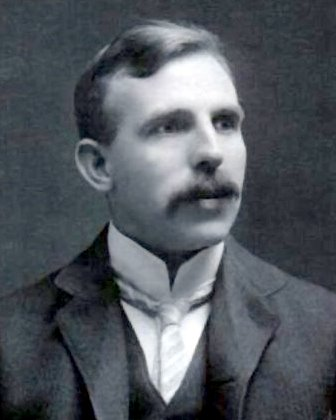
\includegraphics[width=3cm]{01_Introduction/Ernest_Rutherford.jpg}
  \captionsetup{singlelinecheck=off}
  \caption[rutherford]{Ernest Rutherford (1871--1937), physicien d'origine
    néo-zélandaise.
    \begin{itemize}
      \item Travaille à McGill de 1898 à 1907
      \item Prix Nobel de chimie en 1908
      \item Anobli en 1914
      \item Nommé baron de Nelson en 1931
    \end{itemize}
    Citations célèbres:
    ``La science est soit de la physique, soit de la philatélie.''
    ``Une découverte scientifique n'a aucun mérite si elle ne peut être
    expliquée à une serveuse.''}
  \label{fig:rutherford}
\end{marginfigure}

Les forces en question sont \emph{toutes} dues à l'une ou
l'autre des quatres interactions fondamentales :

\begin{itemize}
  \item interaction nucléaire forte
  \item interaction nucléaire faible
  \item interaction électromagnétique
  \item interaction gravitationnelle
\end{itemize}

Les interactions nucléaires fortes et faibles sont responsable de la cohésion
du noyau atomique et de la radioactivité.  La portée de ces interactions est
inférieure à \SI{1e-15}{\meter}, soit de l'ordre de grandeur d'un noyau
atomique.  Bien que très importantes pour expliquer le comportement de la
matière à petite échelle, ces forces sont pratiquement indétectables à notre
échelle.

Les particules qui ont une \textbf{charge électrique} (concept qui sera défini
plus précisément dans le cours \emph{NYB -- Électricité et magnétisme})
interagissent via la force électromagnétique.  La grande majorité des
interactions auxquelles nous sommes habituées sont dues à la force
électromagnétique.  Si vous ne passez pas à travers du plancher, c'est parce
que les électrons sous vos pieds repoussent les électrons à la surface du
plancher.  Le même phénomène explique que vous soyez en mesure de prendre des
objets et de pousser des portes.  La force électromagnétique est également
responsable des réactions chimiques, de la lumière et de la viscosité de l'eau.

Les particules qui ont une \textbf{masse} interagissent via la force
gravitationnelle.  Cette force, à la différence de la force électromagnétique,
est toujours attractive.  La gravité vous retient à la surface de la Terre,
force la Terre à demeurer en orbite autour du Soleil, maintient toutes les
étoiles de la galaxie ensembles et est responsable de la structure à grande
échelle de l'Univers.  Une pomme tombe vers le centre de la Terre à cause de la
gravité et elle s'écrase sur le sol à cause de la force électromagnétique.

Dans le cours de mécanique, nous nous concentrerons sur le mouvement des objets
solides et sur les lois dynamique qui régissent ces mouvements.  L'état de
mouvement d'un objet change s'il est soumis à une \textbf{force} d'un des
quatre types mentionnés plus haut.  Le lois qui décrivent ces forces
elles-mêmes ne seront pas étudiées (sauf pour la gravité), mais nous
développerons les outils qui permettent de comprendre l'effet d'une force.

À plusieurs reprises, nous parlerons de \textbf{particule}.  Une particule peut
être soit une \textbf{particule élémentaire} (par exemple, un électron, un
quark, un gluon, etc.) ou un objet dont les dimensions et les mouvements
internes sont négligeables dans le contexte du problème.
\marginnote{Benson, p. 40}
\marginnote{Reconnaître les situations dans lesquelles on peut faire cette
approximation est une des qualités essentielle du physicien.  La physique est
en quelque sorte l'art de remplacer un problème complexe par un problème plus
simple.}
Souvent, une particule est donc un modèle abstrait d'un objet matériel qu'on
utilise pour simplifier l'analyse.  Par exemple, dans l'étude du mouvement des
planètes autour du Soleil, la taille des planètes est complètement négligeable
et on peut les considérer comme des points.


\section{Les grandeurs fondamentales de la mécanique et les référentiels}

Rappelez-vous qu'un des sujets principaux du cours de mécanique est l'étude du
mouvement.  De quoi a-t-on besoin pour décrire un mouvement?  Qu'est-ce que le
mouvement?  \marginnote{Laisser les étudiants répondre.  Lancer un objet (un
  toutou d'Einstein peut-être) pour les inspirer.}  En y réfléchissant un peu,
vous arrivez probablement à une définition qui se rapproche de la suivante :
\textbf{un objet est en mouvement si sa position change au fil du temps}.
Pour que cette définition toute simple soit complète, on doit préciser trois
quantités fondamentales : la quantité de matière dans l'objet, la position, et
le temps.

Pour fixer les idées, imaginons qu'on parle d'un objet bien spécifique, soit
l'ourson en peluche que je vous montre à l'instant.

\begin{marginfigure}
  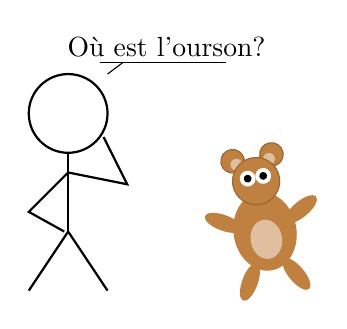
\begin{tikzpicture}[scale=0.5]
    \begin{scope}[shift={(5, 1)}, rotate=10] % Teddy bear
      \teddybear
    \end{scope}
    \begin{scope} % Character
      \draw[thick] (0, 1) -- (0, 3);
      \draw[thick] (0, 1) -- (-1, -0.5);
      \draw[thick] (0, 1) -- (1, -0.5);
      \draw[thick] (0, 4) circle (1);
      \draw[thick] (0, 2.5) -- (1.5, 2.2) -- (0.9, 3.4);
      \draw[thick] (0, 2.5) -- (-1, 1.5) -- (-0.1, 1);
      \draw (1, 5) -- (1.4, 5.3);
      \draw (0.8, 5.3) -- (4, 5.3);
      \node at (2.5, 5.7) {Où est l'ourson?};
    \end{scope}
  \end{tikzpicture}
\end{marginfigure}

\subsection{La masse}

Notre ourson est composé de peluche, de coton et de fibres synthétiques.  On
peut caractériser l'objet par sa taille, sa forme, sa densité, sa couleur, etc.
Dans le cours de mécanique, la plupart du temps, la seule caractéristique
intrinsèque des objets qui nous intéressera est la quantité de matière qui
compose l'objet.  \marginnote{Attention!  L'unité de base est le
  \textbf{kilo}gramme, pas le gramme.}  La quantité de matière est donnée par
la \textbf{masse}.  L'unité de mesure du Système international d'unités (SI)
pour la masse est le \textbf{kilogramme}.  Le symbole utilisé pour le
kilogramme est \textbf{kg}.

\subsection{Le temps}

Pour mesurer le temps, il faut que des événements se produisent.  Par exemple,
on peut définir l'unité de temps \emph{splork} comme l'intervalle entre deux
claquements de doigts, ou entre deux levers de soleil.  Pour que notre unité de
temps soit utile, il faut que les événements se produisent à intervalles
réguliers.  Un dispositif pour mesurer le temps est appelé une horloge.

Dans le SI, le \textbf{temps} est mesuré en \textbf{secondes}.
\marginnote{Attention! Le symbole pour la seconde est s, pas sec.} Une seconde
est définie à partir des oscillations d'un atome de césium 133.  Le symbole
utilisé pour le seconde est \textbf{s}.

\subsection{La longueur}

Pour mesurer une longueur, on doit avoir deux points de référence.  Par
exemple, un des points de référence peut être moi, et l'autre point, l'ourson.
On pourrait définir l'unité de longueur comme la distance entre l'ourson et
moi.  Quiconque veut mesurer une longueur n'a qu'à comparer la longueur désirée
avec la distance entre l'ourson et le prof.  Par exemple, la salle de classe
mesure 8 oursons-profs.

Évidemment, cette définition n'est pas très utile parce qu'il est extrêmement
\marginnote{Dans le cours \emph{NYC - Ondes et physique moderne} vous
  apprendrez que la vitesse de la lumière dans le vide est une constante.
  C'est un des deux postulats de la relativité restreinte.} difficile de
reproduire la distance exacte entre l'ourson et le prof.  L'unité de longueur
dans le SI, le \textbf{mètre}, est la distance parcourue par la lumière dans le
vide en une seconde.  Le symbole utilisé pour le mètre est \textbf{m}.

\subsection{Autres grandeurs}

Le SI contient sept unités de base qui sont décrites dans le tableau
ci-dessous.\marginnote{Attention! Dimension n'a pas le même sens ici que
  lorsqu'on parle d'un espace à trois dimension, ou d'un mouvement à deux
  dimensions.}  On note que dans ce contexte \textbf{dimension} est une
grandeur physique.

\vspace{0.3cm}
\begin{tabular}{lll}
  \toprule
  Dimension              &  Unité       &  Symbole \\
  \midrule
  Longueur               &  mètre       &  m       \\
  Masse                  &  kilogramme  &  kg      \\
  Temps                  &  seconde     &  s       \\
  Courant électrique     &  ampère      &  A       \\
  Température            &  kelvin      &  K       \\
  Quantité de substance  &  mole        &  mol     \\
  Intensité lumineuse    &  candela     &  cd      \\
  \bottomrule
\end{tabular}
\vspace{0.3cm}

En plus des unités de base, il existe un grand nombre d'\textbf{unités
  dérivées} qui sont construites en combinant les unités de base.  Un exemple
avec lequel nous aurons souvent à travailler est la vitesse.  La vitesse est le
taux de variation de la position en fonction du temps, donc son unité est le
\si{\meter\per\second}.  L'unité de force, le newton, est aussi une unité
dérivée : $\SI{1}{\newton} = \SI{1}{\kilogram\meter\per\second\squared}$.
D'autres exemples d'unités dérivées sont l'aire (\si{\meter\squared}), le
volume (\si{\meter\cubed}) et la masse volumique
(\si{\kilogram\per\meter\cubed}).


\subsection{La notation scientifique et les chiffres significatifs}

La physique étudie des phénomènes qui se produisent à l'échelle atomique et à
l'échelle de l'Univers entier, et qui se déroulent sur des périodes de l'ordre
du milliardième de seconde jusqu'au milliard d'années.  Les ordres de grandeurs
considérés sont tels qu'il faut une notation compacte pour représenter les
nombres qu'on considère.  Cette notation est la \textbf{notation scientifique}.
Un nombre en notation scientifique s'écrit
\begin{equation*}
  a,bcd\ldots \times 10^n
\end{equation*}
Par exemple, en utilisant la notation scientifique, \SI{354.24}{\meter} s'écrit
\SI{3.5424e2}{\meter}.

Si quelqu'un vous dit que sa masse est \SI{68.942841}{\kilogram}, il
sous-entend que la précision de sa mesure est très grande!  Il fait la
distinction entre \SI{68.942841}{\kilogram} et \SI{68.942842}{\kilogram}, donc
sa mesure est au moins précise jusqu'à la sixième décimale (soit au
milligramme).  Le problème, c'est que très peu de pèse-personnes permettent de
faire une mesure aussi précise.  
\marginnote{Dans les exercices et les examens, on supposera que toutes les
  quantités sont suffisamment précise pour que les réponses puissent être
  données avec trois chiffres significatifs.}
Quand on donne une valeur numérique, le nombre
de décimales indique à quel point la mesure est précise.  Ainsi,
\SI{68.2}{\kilogram} et \SI{68.200}{\kilogram} n'ont pas la même signification:
la deuxième mesure est précise au gramme, alors que la première n'est précise
qu'au \SI{100}{\gram}.  Le nombre de \textbf{chiffres significatifs} indique à
quel point une mesure est précise.


\subsection{Exemple de conversion d'unités : les deux par quatre}

\exemple{En charpenterie les morceaux de bois deux par quatre sont souvent
  utilisée.  Un tel morceau de bois est un prisme rectangulaire dont la base
  est un rectangle de deux pouces de largeur et de quatre pouces de longueur.
Sachant qu'un pouce est égal à \SI{2.54}{\centi\meter}, déterminer l'aire de la
base en mètres carrés.

\vspace{0.3cm}

Soit $l = \SI{2.00}{pouces}$ la largeur du morceau de bois et $L =
\SI{4.00}{pouces}$ sa longueur.  L'aire de la base, $A$, est le produit de la
longueur et de la largeur.  Par conséquent,
\begin{align*}
  A &= lL \\
    &= \SI{2.00}{pouce} \times \SI{4.00}{pouce} \\
    &= \SI{8.00}{pouce\squared} 
\end{align*}
Pour passer des pouces carrés à des mètres carrés, nous devons d'abord
convertir les pouces en centimètres avec le facteur de conversion donné, puis
convertir de centimètre à mètre en utilisant le fait qu'il y a cent centimètres
dans un mètre.  Une stratégie efficace est de multiplier la valeur numérique
par 1.
\begin{align*}
  A &= \SI{8.00}{pouce\squared} \\
    &= \SI{8.00}{pouce\squared} \times
         \left(\frac{\SI{2.54}{\centi\meter}}{\SI{1}{pouce}}\right)^2 \\
    &= \SI{8.00}{pouce\squared} \times \left(
         \frac{\SI{2.54}{\centi\meter}}{\SI{1}{pouce}}
         \times \frac{\SI{1}{\meter}}{\SI{100}{\centi\meter}}
       \right)^2 \\
    &= \frac{8,00 \times 2,54^2}{100^2} \si{\meter\squared} \\
    &= \SI{5.16e-3}{\meter\squared}
\end{align*}
Une stratégie tout aussi valide est de convertir la longueur et la largeur en
mètres, puis de multiplier les deux valeurs pour obtenir l'aire.
}

\subsection{Exemple de conversion d'unités : élimination métabolique de
  l'alcool}

\exemple{Le taux auquel l'alcool est éliminé du sang est en moyenne
  \SI{15.0}{\milli\gram\per\deci\liter\per\hour}.  Exprimer ce taux en unités
  SI en utilisant la notation scientifique.

  \vspace{0.3cm}

  Il y a plusieurs conversions à faire ici.  D'abord on veut convertir les
  milligrammes en grammes, ensuite les décilitres en mètres cubes, puis les
  heures en secondes.

  \begin{align*}
    \SI{15.0}{\milli\gram\per\deci\liter\per\hour} &=
      \SI{15.0}{\milli\gram\per\deci\liter\per\hour} \times
      \frac{\SI{1}{\kilogram}}{\SI{1e6}{\milli\gram}} \times
      \frac{\SI{10}{\deci\liter}}{\SI{1}{\liter}} \times
      \frac{\SI{1}{\hour}}{\SI{3600}{\second}} \\
    &= 
      \frac{15,0}{\num{3.60e8}}
      \frac{\si{\kilogram}}{\si{\liter\second}} \\
    &= \num{4.16667e-8} \frac{\si{\kilogram}}{\si{\liter\second}} \times
      \frac{\SI{1}{\liter}}{\SI{1}{\deci\meter\cubed}} \\
    &= \num{4.16667e-8} \frac{\si{\kilogram}}{\si{\second}} \times
      \left(\frac{1}{\SI{1}{\deci\meter}} \times
        \frac{\SI{10}{\deci\meter}}{\SI{1}{\meter}}\right)^3 \\
    &= \SI{4.17e-5}{\kilogram\per\meter\cubed\per\second}
  \end{align*}
}


\subsection{Référentiel et système de coordonnées}

Revenons à notre ourson.  Nous savons maintenant ce qu'est la masse et le
temps, mais il reste à définir la position.  Cette dernière est étroitement
liée à la longueur, mais une seule longueur n'est pas suffisante, en général,
pour décrire une position.

Comment peut-on définir une position?  De quoi a-t-on
besoin? On peut pointer du doigt et crier ``là! là!'', mais cela ne décrit pas
très clairement une position, ou du moins, la description est incomplète.  Le
doigt pointé indique dans quelle direction le point d'intérêt se trouve, mais
ne donne aucune indication sur la distance à laquelle il se trouve.  Par
contre, si on pointe du doigt en disant ``l'ourson se trouve à trois mètres'',
alors on a une description précise et complète.

\begin{marginfigure}
  \begin{tikzpicture}[scale=3]
    \coordinate (origin) at (0, 0, 0);
    \coordinate (teddyx) at (0, 0, 0.4);
    \coordinate (teddyy) at (0.6, 0, 0);
    \coordinate (teddyz) at (0, 0.7, 0);
    \coordinate (teddy) at ($(teddyx) + (teddyy) + (teddyz)$);
    \draw[->] (origin) -- (1, 0, 0) node[right] {$y$};
    \draw[->] (origin) -- (0, 1, 0) node[left] {$z$};
    \draw[->] (origin) -- (0, 0, 1) node[anchor=north east] {$x$};
    \begin{scope}[shift={(teddy)}, scale=0.05]
      \teddybear
    \end{scope}
    \draw[->, very thick] (origin) -- (teddy);
    \draw[dotted] (origin) -- ++($(teddyx) + (teddyy)$) -- ++(teddyz);
    \draw[dotted] (teddyz) -- ++($(teddyx) + (teddyy)$);
    \draw (-0.12, -0.12) arc (-80:-45:0.6 and 0.2);
    \node at (0.25, 0, 0.45) {$\varphi$};
    \draw (0, 0.25, 0) arc (90:50:0.25);
    \node at (0.12, 0.3) {$\theta$};
  \end{tikzpicture}
\end{marginfigure}

En pointant du doigt, on accomplit plusieurs choses.  D'abord, on définit un
point de référence, soit l'épaule du pointeur.  Ensuite, on spécifie deux
angles : un \textbf{angle azimutal}, $\varphi$, entre une direction
particulière (disons le Nord) et l'ourson, et un \textbf{angle d'élévation},
$\theta$, par rapport à l'horizontale.  Enfin, en donnant la \textbf{distance}
par rapport au point de référence on spécifie la position de l'ourson sans
aucune ambigüité.

Il y a d'autres approches valides.  Par exemple, on peut spécifier la distance
\marginnote{On remarque que dans les deux cas, il faut trois nombres pour
  décrire une position.  C'est pour cette raison qu'on dit que le monde dans
  lequel nous vivons est à trois dimensions.} à partir de la porte de la classe
en longeant un premier mur (on peut s'imaginer un axe imaginaire le long de ce
mur et l'appeler $x$), puis une distance parallèle aux autres murs (en
direction d'un axe $y$) et enfin une hauteur (l'axe $z$).  Ces trois valeurs
spécifient aussi la position de l'ourson de façon tout à fait claire.

Chacune de ces façons de procéder correspond à un \textbf{système de
  coordonnées}.  Dans le premier cas, ce sont les \textbf{coordonnées
  sphériques}, et dans le deuxième cas, les \textbf{coordonnées cartésiennes}.
Un système de coordonnées est un système qui permet de repérer des points dans
l'espace à l'aide de nombres.  \marginnote{Benson, p. 15} Dans le cours, nous
n'étudierons que des problèmes à une dimension et à deux dimensions.

En physique, un système de coordonnées n'existe jamais dans un néant absolu.
Il est toujours défini dans un référentiel.  Un \textbf{référentiel} est un
système de référence matériel, comme la salle de classe, l'intérieur d'un
ascenseur ou une table de laboratoire.  Dans un même référentiel, on peut
définir plusieurs systèmes de coordonnées.

Deux systèmes de coordonnées à deux dimensions seront particulièrement utiles
dans le cours : le système cartésien et le système polaire.

\begin{marginfigure}
  
\end{marginfigure}

\fullwidth{
\subsection{Exemple de conversion du système de coordonnées cartésiennes au
  système de coordonnées polaires}
}

\exemple{

}

